% Options for packages loaded elsewhere
\PassOptionsToPackage{unicode}{hyperref}
\PassOptionsToPackage{hyphens}{url}
\PassOptionsToPackage{dvipsnames,svgnames,x11names}{xcolor}
%
\documentclass[
  letterpaper,
  DIV=11,
  numbers=noendperiod]{scrartcl}

\usepackage{amsmath,amssymb}
\usepackage{iftex}
\ifPDFTeX
  \usepackage[T1]{fontenc}
  \usepackage[utf8]{inputenc}
  \usepackage{textcomp} % provide euro and other symbols
\else % if luatex or xetex
  \usepackage{unicode-math}
  \defaultfontfeatures{Scale=MatchLowercase}
  \defaultfontfeatures[\rmfamily]{Ligatures=TeX,Scale=1}
\fi
\usepackage{lmodern}
\ifPDFTeX\else  
    % xetex/luatex font selection
\fi
% Use upquote if available, for straight quotes in verbatim environments
\IfFileExists{upquote.sty}{\usepackage{upquote}}{}
\IfFileExists{microtype.sty}{% use microtype if available
  \usepackage[]{microtype}
  \UseMicrotypeSet[protrusion]{basicmath} % disable protrusion for tt fonts
}{}
\makeatletter
\@ifundefined{KOMAClassName}{% if non-KOMA class
  \IfFileExists{parskip.sty}{%
    \usepackage{parskip}
  }{% else
    \setlength{\parindent}{0pt}
    \setlength{\parskip}{6pt plus 2pt minus 1pt}}
}{% if KOMA class
  \KOMAoptions{parskip=half}}
\makeatother
\usepackage{xcolor}
\setlength{\emergencystretch}{3em} % prevent overfull lines
\setcounter{secnumdepth}{-\maxdimen} % remove section numbering
% Make \paragraph and \subparagraph free-standing
\ifx\paragraph\undefined\else
  \let\oldparagraph\paragraph
  \renewcommand{\paragraph}[1]{\oldparagraph{#1}\mbox{}}
\fi
\ifx\subparagraph\undefined\else
  \let\oldsubparagraph\subparagraph
  \renewcommand{\subparagraph}[1]{\oldsubparagraph{#1}\mbox{}}
\fi

\usepackage{color}
\usepackage{fancyvrb}
\newcommand{\VerbBar}{|}
\newcommand{\VERB}{\Verb[commandchars=\\\{\}]}
\DefineVerbatimEnvironment{Highlighting}{Verbatim}{commandchars=\\\{\}}
% Add ',fontsize=\small' for more characters per line
\usepackage{framed}
\definecolor{shadecolor}{RGB}{241,243,245}
\newenvironment{Shaded}{\begin{snugshade}}{\end{snugshade}}
\newcommand{\AlertTok}[1]{\textcolor[rgb]{0.68,0.00,0.00}{#1}}
\newcommand{\AnnotationTok}[1]{\textcolor[rgb]{0.37,0.37,0.37}{#1}}
\newcommand{\AttributeTok}[1]{\textcolor[rgb]{0.40,0.45,0.13}{#1}}
\newcommand{\BaseNTok}[1]{\textcolor[rgb]{0.68,0.00,0.00}{#1}}
\newcommand{\BuiltInTok}[1]{\textcolor[rgb]{0.00,0.23,0.31}{#1}}
\newcommand{\CharTok}[1]{\textcolor[rgb]{0.13,0.47,0.30}{#1}}
\newcommand{\CommentTok}[1]{\textcolor[rgb]{0.37,0.37,0.37}{#1}}
\newcommand{\CommentVarTok}[1]{\textcolor[rgb]{0.37,0.37,0.37}{\textit{#1}}}
\newcommand{\ConstantTok}[1]{\textcolor[rgb]{0.56,0.35,0.01}{#1}}
\newcommand{\ControlFlowTok}[1]{\textcolor[rgb]{0.00,0.23,0.31}{#1}}
\newcommand{\DataTypeTok}[1]{\textcolor[rgb]{0.68,0.00,0.00}{#1}}
\newcommand{\DecValTok}[1]{\textcolor[rgb]{0.68,0.00,0.00}{#1}}
\newcommand{\DocumentationTok}[1]{\textcolor[rgb]{0.37,0.37,0.37}{\textit{#1}}}
\newcommand{\ErrorTok}[1]{\textcolor[rgb]{0.68,0.00,0.00}{#1}}
\newcommand{\ExtensionTok}[1]{\textcolor[rgb]{0.00,0.23,0.31}{#1}}
\newcommand{\FloatTok}[1]{\textcolor[rgb]{0.68,0.00,0.00}{#1}}
\newcommand{\FunctionTok}[1]{\textcolor[rgb]{0.28,0.35,0.67}{#1}}
\newcommand{\ImportTok}[1]{\textcolor[rgb]{0.00,0.46,0.62}{#1}}
\newcommand{\InformationTok}[1]{\textcolor[rgb]{0.37,0.37,0.37}{#1}}
\newcommand{\KeywordTok}[1]{\textcolor[rgb]{0.00,0.23,0.31}{#1}}
\newcommand{\NormalTok}[1]{\textcolor[rgb]{0.00,0.23,0.31}{#1}}
\newcommand{\OperatorTok}[1]{\textcolor[rgb]{0.37,0.37,0.37}{#1}}
\newcommand{\OtherTok}[1]{\textcolor[rgb]{0.00,0.23,0.31}{#1}}
\newcommand{\PreprocessorTok}[1]{\textcolor[rgb]{0.68,0.00,0.00}{#1}}
\newcommand{\RegionMarkerTok}[1]{\textcolor[rgb]{0.00,0.23,0.31}{#1}}
\newcommand{\SpecialCharTok}[1]{\textcolor[rgb]{0.37,0.37,0.37}{#1}}
\newcommand{\SpecialStringTok}[1]{\textcolor[rgb]{0.13,0.47,0.30}{#1}}
\newcommand{\StringTok}[1]{\textcolor[rgb]{0.13,0.47,0.30}{#1}}
\newcommand{\VariableTok}[1]{\textcolor[rgb]{0.07,0.07,0.07}{#1}}
\newcommand{\VerbatimStringTok}[1]{\textcolor[rgb]{0.13,0.47,0.30}{#1}}
\newcommand{\WarningTok}[1]{\textcolor[rgb]{0.37,0.37,0.37}{\textit{#1}}}

\providecommand{\tightlist}{%
  \setlength{\itemsep}{0pt}\setlength{\parskip}{0pt}}\usepackage{longtable,booktabs,array}
\usepackage{calc} % for calculating minipage widths
% Correct order of tables after \paragraph or \subparagraph
\usepackage{etoolbox}
\makeatletter
\patchcmd\longtable{\par}{\if@noskipsec\mbox{}\fi\par}{}{}
\makeatother
% Allow footnotes in longtable head/foot
\IfFileExists{footnotehyper.sty}{\usepackage{footnotehyper}}{\usepackage{footnote}}
\makesavenoteenv{longtable}
\usepackage{graphicx}
\makeatletter
\def\maxwidth{\ifdim\Gin@nat@width>\linewidth\linewidth\else\Gin@nat@width\fi}
\def\maxheight{\ifdim\Gin@nat@height>\textheight\textheight\else\Gin@nat@height\fi}
\makeatother
% Scale images if necessary, so that they will not overflow the page
% margins by default, and it is still possible to overwrite the defaults
% using explicit options in \includegraphics[width, height, ...]{}
\setkeys{Gin}{width=\maxwidth,height=\maxheight,keepaspectratio}
% Set default figure placement to htbp
\makeatletter
\def\fps@figure{htbp}
\makeatother

\KOMAoption{captions}{tableheading}
\makeatletter
\makeatother
\makeatletter
\makeatother
\makeatletter
\@ifpackageloaded{caption}{}{\usepackage{caption}}
\AtBeginDocument{%
\ifdefined\contentsname
  \renewcommand*\contentsname{Table of contents}
\else
  \newcommand\contentsname{Table of contents}
\fi
\ifdefined\listfigurename
  \renewcommand*\listfigurename{List of Figures}
\else
  \newcommand\listfigurename{List of Figures}
\fi
\ifdefined\listtablename
  \renewcommand*\listtablename{List of Tables}
\else
  \newcommand\listtablename{List of Tables}
\fi
\ifdefined\figurename
  \renewcommand*\figurename{Figure}
\else
  \newcommand\figurename{Figure}
\fi
\ifdefined\tablename
  \renewcommand*\tablename{Table}
\else
  \newcommand\tablename{Table}
\fi
}
\@ifpackageloaded{float}{}{\usepackage{float}}
\floatstyle{ruled}
\@ifundefined{c@chapter}{\newfloat{codelisting}{h}{lop}}{\newfloat{codelisting}{h}{lop}[chapter]}
\floatname{codelisting}{Listing}
\newcommand*\listoflistings{\listof{codelisting}{List of Listings}}
\makeatother
\makeatletter
\@ifpackageloaded{caption}{}{\usepackage{caption}}
\@ifpackageloaded{subcaption}{}{\usepackage{subcaption}}
\makeatother
\makeatletter
\@ifpackageloaded{tcolorbox}{}{\usepackage[skins,breakable]{tcolorbox}}
\makeatother
\makeatletter
\@ifundefined{shadecolor}{\definecolor{shadecolor}{rgb}{.97, .97, .97}}
\makeatother
\makeatletter
\makeatother
\makeatletter
\makeatother
\ifLuaTeX
  \usepackage{selnolig}  % disable illegal ligatures
\fi
\IfFileExists{bookmark.sty}{\usepackage{bookmark}}{\usepackage{hyperref}}
\IfFileExists{xurl.sty}{\usepackage{xurl}}{} % add URL line breaks if available
\urlstyle{same} % disable monospaced font for URLs
\hypersetup{
  pdftitle={Single Cell Analysis of Cite-seq data},
  pdfauthor={Max Mattessich, Joaquin Reyna, Edel Aron, Anna Konstorum},
  colorlinks=true,
  linkcolor={blue},
  filecolor={Maroon},
  citecolor={Blue},
  urlcolor={Blue},
  pdfcreator={LaTeX via pandoc}}

\title{Single Cell Analysis of Cite-seq data}
\author{Max Mattessich, Joaquin Reyna, Edel Aron, Anna Konstorum}
\date{2023-04-06}

\begin{document}
\maketitle
\ifdefined\Shaded\renewenvironment{Shaded}{\begin{tcolorbox}[breakable, frame hidden, boxrule=0pt, enhanced, sharp corners, interior hidden, borderline west={3pt}{0pt}{shadecolor}]}{\end{tcolorbox}}\fi

\hypertarget{introduction}{%
\subsection{Introduction}\label{introduction}}

In this vignette, we will cover some of the possible sources for
publicly available single-cell data, how to format it for and process it
with MCIA and how to run a basic analysis in order to annotate the data
and use the results as metadata for exploring the decomposition results.

\textbf{\texttt{OUTLINE}}

\includegraphics{citeseq_files/mediabag/uc-export=view-id=1t.pdf}

\textbf{\texttt{DATA\ FLOW}}

\includegraphics[width=19.44792in,height=\textheight]{citeseq_files/mediabag/uc-export=view-id=1r.pdf}

\includegraphics{citeseq_files/mediabag/uc-export=view-id=1h.pdf}

\begin{Shaded}
\begin{Highlighting}[]
\FunctionTok{library}\NormalTok{(dplyr)}
\end{Highlighting}
\end{Shaded}

\begin{verbatim}

Attaching package: 'dplyr'
\end{verbatim}

\begin{verbatim}
The following objects are masked from 'package:stats':

    filter, lag
\end{verbatim}

\begin{verbatim}
The following objects are masked from 'package:base':

    intersect, setdiff, setequal, union
\end{verbatim}

\begin{Shaded}
\begin{Highlighting}[]
\FunctionTok{library}\NormalTok{(ggplot2)}
\FunctionTok{library}\NormalTok{(ggpubr)}
\FunctionTok{library}\NormalTok{(Seurat)}
\end{Highlighting}
\end{Shaded}

\begin{verbatim}
Attaching SeuratObject
\end{verbatim}

\hypertarget{data}{%
\subsection{Data}\label{data}}

We will be using the 10x Genomics ``pbmc5k-CITEseq'' dataset, which was
published in May 2019 and processed using Cell Ranger 3.0.2. It contains
5,247 detected cells from PBMCs and 33,538 genes along with 32 cell
surface markers. We chose this dataset due to it containing both gene
expression (GEX) and cell surface protein (ADT) data as well as being
publicly available and from a widely used platform.

The following code details several ways in which to load in this
dataset. The original dataset can be found on the
{[}\href{https://support.10xgenomics.com/single-cell-gene-expression/datasets/3.0.2/5k_pbmc_protein_v3}{10x
Genomics Datasets website}{]} and an explanation of the file types for
this version can be found
\href{https://support.10xgenomics.com/single-cell-gene-expression/software/pipelines/3.0/output/overview}{here}.
You can download them all to a directory of your choosing with their
suggested terminal commands:

\begin{Shaded}
\begin{Highlighting}[]
\FunctionTok{getwd}\NormalTok{()}
\end{Highlighting}
\end{Shaded}

\begin{verbatim}
[1] "C:/Users/ferhatay/Desktop/BGGN239-Week2-Ferhat/singleCell-Vignette/vignettes"
\end{verbatim}

\begin{verbatim}
[1] "C:/Users/ferhatay/Desktop/BGGN239-Week2-Ferhat/singleCell-Vignette/vignettes"
\end{verbatim}

\begin{verbatim}
[1] "../data"
\end{verbatim}

If you would like to view some basic information about the data, you can
open the *web\_summary.html* in your favorite web browser. It will show
the estimated number of cells, mean reads per cell, median genes per
cell and a variety of other sample metrics. These metrics are also
available in the *metrics\_summary.csv*

You will need the *filtered\_feature\_bc\_matrix* directory for the
following analysis; it can be extracted with `tar -xvzf
5k\_pbmc\_protein\_v3\_filtered\_feature\_bc\_matrix.tar.gz` from within
the relevant data directory. Or can be done in R as below:

\hypertarget{extract-the-data}{%
\subsubsection{Extract the data}\label{extract-the-data}}

\begin{Shaded}
\begin{Highlighting}[]
\CommentTok{\# Extract the data}
\ControlFlowTok{if}\NormalTok{ (}\SpecialCharTok{!}\FunctionTok{file.exists}\NormalTok{(}\FunctionTok{file.path}\NormalTok{(path\_data, }\StringTok{"tenx\_pbmc5k\_CITEseq"}\NormalTok{)))\{}

\NormalTok{tar\_fn }\OtherTok{=} \FunctionTok{file.path}\NormalTok{(path\_data, }\StringTok{"5k\_pbmc\_protein\_v3\_filtered\_feature\_bc\_matrix.tar.gz"}\NormalTok{)}
\CommentTok{\#exdir = file.path(path\_data, "5k\_pbmc\_protein\_v3\_filtered\_feature\_bc\_matrix")}
\NormalTok{exdir }\OtherTok{=} \FunctionTok{file.path}\NormalTok{(path\_data, }\StringTok{"tenx\_pbmc5k\_CITEseq"}\NormalTok{)}
\FunctionTok{untar}\NormalTok{(tar\_fn, }\AttributeTok{exdir =}\NormalTok{ exdir, }\AttributeTok{tar =} \StringTok{"internal"}\NormalTok{)}
\NormalTok{\}}
\end{Highlighting}
\end{Shaded}

\hypertarget{seurat-analysis}{%
\subsection{Seurat Analysis}\label{seurat-analysis}}

This section demonstrates how to take in raw data (in this case, the
output of Cell Ranger) and go through a popular analysis pipeline to
ultimately cluster and annotate the data. Some people prefer to use Cell
Ranger's built-in dimension reduction and clustering analysis and to
view the results with
\href{https://support.10xgenomics.com/single-cell-gene-expression/software/visualization/latest/what-is-loupe-cell-browser}{Loupe
Cell Browser}.

\emph{Credit to Seurat
(\href{https://satijalab.org/seurat/articles/pbmc3k_tutorial.html}{RNA}
and
\href{https://satijalab.org/seurat/articles/multimodal_vignette.html\#setup-a-seurat-object-add-the-rna-and-protein-data}{multi-modal})
for the general steps.}

\hypertarget{load-the-data-in-to-a-seurat-object}{%
\subsubsection{Load the data in to a Seurat
object}\label{load-the-data-in-to-a-seurat-object}}

\begin{Shaded}
\begin{Highlighting}[]
\CommentTok{\# load the data (change the file path as needed)}
\NormalTok{data }\OtherTok{\textless{}{-}}\NormalTok{ Seurat}\SpecialCharTok{::}\FunctionTok{Read10X}\NormalTok{(}\AttributeTok{data.dir =} \FunctionTok{file.path}\NormalTok{(path\_data, }\StringTok{"tenx\_pbmc5k\_CITEseq"}\NormalTok{,                                        }\StringTok{"filtered\_feature\_bc\_matrix"}\NormalTok{),}
                        \AttributeTok{strip.suffix =} \ConstantTok{TRUE}\NormalTok{) }\CommentTok{\# remove the "{-}1"s from barcodes}
\end{Highlighting}
\end{Shaded}

\begin{verbatim}
10X data contains more than one type and is being returned as a list containing matrices of each type.
\end{verbatim}

\begin{Shaded}
\begin{Highlighting}[]
\DocumentationTok{\#\# 10X data contains more than one type and is being returned as a list}
\DocumentationTok{\#\# containing matrices of each type.}

\CommentTok{\# set minimum cells and/or features here if you\textquotesingle{}d like}
\NormalTok{obj }\OtherTok{\textless{}{-}}\NormalTok{ Seurat}\SpecialCharTok{::}\FunctionTok{CreateSeuratObject}\NormalTok{(}\AttributeTok{counts =}\NormalTok{ data}\SpecialCharTok{$}\StringTok{\textasciigrave{}}\AttributeTok{Gene Expression}\StringTok{\textasciigrave{}}\NormalTok{,}
                                  \AttributeTok{project =} \StringTok{"pbmc5k\_CITEseq"}\NormalTok{)}
\NormalTok{obj[[}\StringTok{"ADT"}\NormalTok{]] }\OtherTok{\textless{}{-}}\NormalTok{ Seurat}\SpecialCharTok{::}\FunctionTok{CreateAssayObject}\NormalTok{(}\AttributeTok{counts =}\NormalTok{ data}\SpecialCharTok{$}\StringTok{\textasciigrave{}}\AttributeTok{Antibody Capture}\StringTok{\textasciigrave{}}\NormalTok{)}
\end{Highlighting}
\end{Shaded}

\begin{verbatim}
Warning: Feature names cannot have underscores ('_'), replacing with dashes
('-')
\end{verbatim}

\begin{Shaded}
\begin{Highlighting}[]
\DocumentationTok{\#\# Warning: Feature names cannot have underscores (\textquotesingle{}\_\textquotesingle{}), replacing with dashes (\textquotesingle{}{-}\textquotesingle{})}

\CommentTok{\# check the assays}
\NormalTok{Seurat}\SpecialCharTok{::}\FunctionTok{Assays}\NormalTok{(}\AttributeTok{object =}\NormalTok{ obj)}
\end{Highlighting}
\end{Shaded}

\begin{verbatim}
[1] "RNA" "ADT"
\end{verbatim}

\begin{Shaded}
\begin{Highlighting}[]
\DocumentationTok{\#\# "RNA" "ADT"}

\CommentTok{\# list out the CITE{-}Seq surface protein markers}
\FunctionTok{rownames}\NormalTok{(obj[[}\StringTok{"ADT"}\NormalTok{]])}
\end{Highlighting}
\end{Shaded}

\begin{verbatim}
 [1] "CD3-TotalSeqB"           "CD4-TotalSeqB"          
 [3] "CD8a-TotalSeqB"          "CD11b-TotalSeqB"        
 [5] "CD14-TotalSeqB"          "CD15-TotalSeqB"         
 [7] "CD16-TotalSeqB"          "CD19-TotalSeqB"         
 [9] "CD20-TotalSeqB"          "CD25-TotalSeqB"         
[11] "CD27-TotalSeqB"          "CD28-TotalSeqB"         
[13] "CD34-TotalSeqB"          "CD45RA-TotalSeqB"       
[15] "CD45RO-TotalSeqB"        "CD56-TotalSeqB"         
[17] "CD62L-TotalSeqB"         "CD69-TotalSeqB"         
[19] "CD80-TotalSeqB"          "CD86-TotalSeqB"         
[21] "CD127-TotalSeqB"         "CD137-TotalSeqB"        
[23] "CD197-TotalSeqB"         "CD274-TotalSeqB"        
[25] "CD278-TotalSeqB"         "CD335-TotalSeqB"        
[27] "PD-1-TotalSeqB"          "HLA-DR-TotalSeqB"       
[29] "TIGIT-TotalSeqB"         "IgG1-control-TotalSeqB" 
[31] "IgG2a-control-TotalSeqB" "IgG2b-control-TotalSeqB"
\end{verbatim}

\begin{Shaded}
\begin{Highlighting}[]
\CommentTok{\# list out the RNA gene labels}
\CommentTok{\#rownames(obj[["RNA"]])}
\CommentTok{\#length(colnames(obj))}
\NormalTok{obj}
\end{Highlighting}
\end{Shaded}

\begin{verbatim}
An object of class Seurat 
33570 features across 5247 samples within 2 assays 
Active assay: RNA (33538 features, 0 variable features)
 1 other assay present: ADT
\end{verbatim}

\begin{Shaded}
\begin{Highlighting}[]
\CommentTok{\# add useful metadata to the Seurat object}
\CommentTok{\# in this case the percent of mitochondrial reads}
\NormalTok{obj[[}\StringTok{"percent.mt"}\NormalTok{]] }\OtherTok{\textless{}{-}} \FunctionTok{PercentageFeatureSet}\NormalTok{(}\AttributeTok{object =}\NormalTok{ obj, }\AttributeTok{pattern =} \StringTok{"\^{}MT{-}"}\NormalTok{)}
\end{Highlighting}
\end{Shaded}

\hypertarget{metrics-summary}{%
\paragraph{Metrics summary}\label{metrics-summary}}

\begin{Shaded}
\begin{Highlighting}[]
\CommentTok{\# read in the summary table}
\FunctionTok{getwd}\NormalTok{()}
\end{Highlighting}
\end{Shaded}

\begin{verbatim}
[1] "C:/Users/ferhatay/Desktop/BGGN239-Week2-Ferhat/singleCell-Vignette/vignettes"
\end{verbatim}

\begin{Shaded}
\begin{Highlighting}[]
\FunctionTok{list.files}\NormalTok{(path\_data)}
\end{Highlighting}
\end{Shaded}

\begin{verbatim}
[1] "5k_pbmc_protein_v3_filtered_feature_bc_matrix.tar.gz"
[2] "5k_pbmc_protein_v3_metrics_summary.csv"              
[3] "5k_pbmc_protein_v3_raw_feature_bc_matrix.tar.gz"     
[4] "5k_pbmc_protein_v3_web_summary.html"                 
[5] "a.csv.xlsx"                                          
[6] "marker_genes.csv"                                    
[7] "tenx_pbmc5k_CITEseq"                                 
\end{verbatim}

\begin{Shaded}
\begin{Highlighting}[]
\NormalTok{metrics\_summary }\OtherTok{\textless{}{-}} \FunctionTok{read.csv}\NormalTok{(}
    \AttributeTok{file =} \FunctionTok{file.path}\NormalTok{(path\_data, }\StringTok{"5k\_pbmc\_protein\_v3\_metrics\_summary.csv"}\NormalTok{)}
\NormalTok{    )}
\NormalTok{metrics\_summary }
\end{Highlighting}
\end{Shaded}

\begin{verbatim}
  Estimated.Number.of.Cells Mean.Reads.per.Cell Median.Genes.per.Cell
1                     5,247              28,917                 1,646
  Number.of.Reads Valid.Barcodes Sequencing.Saturation Q30.Bases.in.Barcode
1     151,731,342          97.5%                 52.4%                95.8%
  Q30.Bases.in.RNA.Read Q30.Bases.in.Sample.Index Q30.Bases.in.UMI
1                 91.9%                     89.8%            95.4%
  Reads.Mapped.to.Genome Reads.Mapped.Confidently.to.Genome
1                  94.3%                              88.4%
  Reads.Mapped.Confidently.to.Intergenic.Regions
1                                           6.8%
  Reads.Mapped.Confidently.to.Intronic.Regions
1                                        25.0%
  Reads.Mapped.Confidently.to.Exonic.Regions
1                                      56.7%
  Reads.Mapped.Confidently.to.Transcriptome Reads.Mapped.Antisense.to.Gene
1                                     53.2%                           1.3%
  Fraction.Reads.in.Cells Total.Genes.Detected Median.UMI.Counts.per.Cell
1                   87.7%               20,840                      5,506
  Antibody..Number.of.Reads Antibody..Mean.Reads.per.Cell
1                39,096,673                         7,451
  Antibody..Valid.Barcodes Antibody..Sequencing.Saturation
1                    99.0%                           39.6%
  Antibody..Q30.Bases.in.Barcode Antibody..Q30.Bases.in.Antibody.Read
1                          96.7%                                96.0%
  Antibody..Q30.Bases.in.Sample.Index Antibody..Q30.Bases.in.UMI
1                               87.5%                      96.8%
  Antibody..Fraction.Antibody.Reads Antibody..Fraction.Antibody.Reads.Usable
1                             94.3%                                    67.4%
  Antibody..Antibody.Reads.Usable.per.Cell
1                                    5,022
  Antibody..Fraction.Reads.in.Barcodes.with.High.UMI.Counts
1                                                      0.0%
  Antibody..Fraction.Unrecognized.Antibody Antibody..Antibody.Reads.in.Cells
1                                     5.7%                             72.1%
  Antibody..Median.UMIs.per.Cell..summed.over.all.recognized.antibody.barcodes.
1                                                                         2,757
\end{verbatim}

\hypertarget{gene-expression-quality-control-and-filtering}{%
\paragraph{Gene expression quality control and
filtering}\label{gene-expression-quality-control-and-filtering}}

\begin{Shaded}
\begin{Highlighting}[]
\CommentTok{\# try + vs \& }
\FunctionTok{VlnPlot}\NormalTok{(}\AttributeTok{object =}\NormalTok{ obj,}
        \AttributeTok{features =} \FunctionTok{c}\NormalTok{(}\StringTok{"nFeature\_RNA"}\NormalTok{, }\StringTok{"nCount\_RNA"}\NormalTok{, }\StringTok{"percent.mt"}\NormalTok{),}
        \AttributeTok{pt.size =} \FloatTok{0.01}\NormalTok{, }\AttributeTok{ncol =} \DecValTok{3}\NormalTok{) }\SpecialCharTok{\&} \FunctionTok{labs}\NormalTok{(}\AttributeTok{x=}\StringTok{""}\NormalTok{)}
\end{Highlighting}
\end{Shaded}

\begin{figure}[H]

{\centering 
\includegraphics{citeseq_files/figure-pdf/unnamed-chunk-7-1.pdf}

}

\end{figure}

\begin{Shaded}
\begin{Highlighting}[]
\FunctionTok{dim}\NormalTok{(obj)}
\end{Highlighting}
\end{Shaded}

\begin{verbatim}
[1] 33538  5247
\end{verbatim}

Based on the previous plots, a minimum of 500 features and a maximum of
20\% mitochondrial seemed like good cutoffs.

\begin{Shaded}
\begin{Highlighting}[]
\CommentTok{\# adjust cutoffs as desired}
\CommentTok{\#\& nFeature\_RNA \textless{}4000}
\NormalTok{obj }\OtherTok{\textless{}{-}} \FunctionTok{subset}\NormalTok{(}\AttributeTok{x =}\NormalTok{ obj, }\AttributeTok{subset =}\NormalTok{ nFeature\_RNA }\SpecialCharTok{\textgreater{}} \DecValTok{200}  \SpecialCharTok{\&}\NormalTok{ percent.mt }\SpecialCharTok{\textless{}} \DecValTok{20}\NormalTok{)}

\FunctionTok{VlnPlot}\NormalTok{(}\AttributeTok{object =}\NormalTok{ obj,}
        \AttributeTok{features =} \FunctionTok{c}\NormalTok{(}\StringTok{"nFeature\_RNA"}\NormalTok{, }\StringTok{"nCount\_RNA"}\NormalTok{, }\StringTok{"percent.mt"}\NormalTok{),}
        \AttributeTok{pt.size =} \FloatTok{0.01}\NormalTok{, }\AttributeTok{ncol =} \DecValTok{3}\NormalTok{) }\SpecialCharTok{\&} \FunctionTok{labs}\NormalTok{(}\AttributeTok{x=}\StringTok{""}\NormalTok{)}
\end{Highlighting}
\end{Shaded}

\begin{figure}[H]

{\centering 
\includegraphics{citeseq_files/figure-pdf/unnamed-chunk-8-1.pdf}

}

\end{figure}

\begin{Shaded}
\begin{Highlighting}[]
\FunctionTok{dim}\NormalTok{(obj)}
\end{Highlighting}
\end{Shaded}

\begin{verbatim}
[1] 33538  4193
\end{verbatim}

\hypertarget{seurat-data-normalization-and-transformation}{%
\paragraph{Seurat data normalization and
transformation}\label{seurat-data-normalization-and-transformation}}

\begin{Shaded}
\begin{Highlighting}[]
\CommentTok{\# standard log normalization for RNA and centered log for ADT}
\NormalTok{obj }\OtherTok{\textless{}{-}} \FunctionTok{NormalizeData}\NormalTok{(}\AttributeTok{object =}\NormalTok{ obj, }\AttributeTok{normalization.method =} \StringTok{"LogNormalize"}\NormalTok{,}
                     \AttributeTok{scale.factor =} \DecValTok{10000}\NormalTok{, }\AttributeTok{assay =} \StringTok{"RNA"}\NormalTok{)}
\CommentTok{\# log1p(exp(1){-}1)}

\DocumentationTok{\#\# Normalizing across cells for the ADT data}
\NormalTok{obj }\OtherTok{\textless{}{-}} \FunctionTok{NormalizeData}\NormalTok{(}\AttributeTok{object =}\NormalTok{ obj, }\AttributeTok{normalization.method =} \StringTok{"CLR"}\NormalTok{,}
                     \AttributeTok{margin =} \DecValTok{2}\NormalTok{, }\AttributeTok{assay =} \StringTok{"ADT"}\NormalTok{)  }
\end{Highlighting}
\end{Shaded}

\begin{verbatim}
Normalizing across cells
\end{verbatim}

\begin{Shaded}
\begin{Highlighting}[]
\CommentTok{\#margin=1 is features margin=2 is across cells}

\CommentTok{\# highly variable features}
\CommentTok{\# does it only on the RNA because "Active Assay" is RNA}
\CommentTok{\# can be set by DefaultAssay() function}
\NormalTok{obj }\OtherTok{\textless{}{-}} \FunctionTok{FindVariableFeatures}\NormalTok{(}\AttributeTok{object =}\NormalTok{ obj, }\AttributeTok{selection.method =} \StringTok{"vst"}\NormalTok{,}
                            \AttributeTok{nfeatures =} \DecValTok{2000}\NormalTok{)}

\CommentTok{\# scaling so the average expression is 0 and the variance is 1}
\CommentTok{\# only for RNA component }
\NormalTok{obj }\OtherTok{\textless{}{-}} \FunctionTok{ScaleData}\NormalTok{(}\AttributeTok{object =}\NormalTok{ obj, }\AttributeTok{features =} \FunctionTok{rownames}\NormalTok{(obj))}
\end{Highlighting}
\end{Shaded}

\begin{verbatim}
Centering and scaling data matrix
\end{verbatim}

\begin{Shaded}
\begin{Highlighting}[]
\CommentTok{\#obj@meta.data}
\end{Highlighting}
\end{Shaded}

\hypertarget{principal-component-analysis-pca-and-dimensionality-reduction--fun-stuff}{%
\paragraph{Principal component analysis (PCA) and dimensionality
reduction -FUN
STUFF!}\label{principal-component-analysis-pca-and-dimensionality-reduction--fun-stuff}}

\begin{Shaded}
\begin{Highlighting}[]
\CommentTok{\# dimensionality reduction}
\NormalTok{obj }\OtherTok{\textless{}{-}} \FunctionTok{RunPCA}\NormalTok{(}\AttributeTok{object =}\NormalTok{ obj)}
\end{Highlighting}
\end{Shaded}

\begin{verbatim}
PC_ 1 
Positive:  LYZ, FCN1, CST3, MNDA, CTSS, PSAP, S100A9, FGL2, AIF1, GRN 
       NCF2, LST1, CD68, TYMP, SERPINA1, CYBB, CLEC12A, CSTA, SPI1, TNFAIP2 
       CPVL, VCAN, MPEG1, TYROBP, KLF4, FTL, S100A8, IGSF6, CD14, MS4A6A 
Negative:  CD3D, TRAC, LTB, TRBC2, IL32, CD3G, IL7R, CD69, CD247, TRBC1 
       CD2, CD7, CD27, ARL4C, ISG20, HIST1H4C, SYNE2, GZMM, ITM2A, CCR7 
       RORA, MAL, CXCR4, LEF1, TRAT1, CTSW, GZMA, KLRB1, TRABD2A, CCL5 
PC_ 2 
Positive:  CD79A, MS4A1, IGHM, BANK1, HLA-DQA1, CD79B, IGKC, LINC00926, RALGPS2, TNFRSF13C 
       VPREB3, IGHD, SPIB, CD22, FCRL1, HLA-DQB1, BLK, FAM129C, FCRLA, TCL1A 
       GNG7, TCF4, COBLL1, PAX5, SWAP70, CD40, BCL11A, P2RX5, TSPAN13, ADAM28 
Negative:  NKG7, CST7, GZMA, PRF1, KLRD1, CTSW, FGFBP2, GNLY, GZMH, CCL5 
       GZMM, CD247, KLRF1, HOPX, SPON2, ADGRG1, TRDC, MATK, GZMB, FCGR3A 
       S100A4, CCL4, CLIC3, KLRB1, IL2RB, TBX21, TTC38, ANXA1, PTGDR, PLEKHF1 
PC_ 3 
Positive:  GZMB, NKG7, GNLY, CLIC3, PRF1, KLRD1, FGFBP2, KLRF1, SPON2, CST7 
       GZMH, FCGR3A, ADGRG1, GZMA, HOPX, CTSW, TRDC, CCL4, HLA-DPB1, C12orf75 
       PLAC8, TTC38, PLEK, APOBEC3G, TBX21, PRSS23, CYBA, MATK, SYNGR1, CXXC5 
Negative:  IL7R, MAL, LEF1, TRABD2A, TRAC, CCR7, LTB, CD27, FOS, LRRN3 
       FHIT, TRAT1, RGCC, CAMK4, CD3D, RGS10, CD40LG, FOSB, AQP3, SOCS3 
       FLT3LG, CD3G, SLC2A3, TSHZ2, VIM, S100A12, S100A8, CD28, PLK3, VCAN 
PC_ 4 
Positive:  FCER1A, PLD4, SERPINF1, IL3RA, CLEC10A, GAS6, LILRA4, TPM2, CLEC4C, ENHO 
       FLT3, SMPD3, ITM2C, LGMN, CD1C, P2RY14, PPP1R14B, SCT, PROC, LAMP5 
       RUNX2, AC119428.2, PACSIN1, DNASE1L3, PTCRA, RGS10, UGCG, CLIC2, PPM1J, P2RY6 
Negative:  MS4A1, CD79A, LINC00926, BANK1, TNFRSF13C, VPREB3, CD79B, RALGPS2, IGHD, FCRL1 
       BLK, IGHM, CD22, PAX5, ARHGAP24, CD24, P2RX5, NCF1, S100A12, CD19 
       SWAP70, FCRLA, VNN2, TNFRSF13B, FCER2, IGKC, FCRL2, RBP7, CD40, S100A8 
PC_ 5 
Positive:  BATF3, C1QA, TCF7L2, CTSL, CDKN1C, HLA-DQB1, HES4, SIGLEC10, CLEC10A, ABI3 
       HLA-DQA1, RHOC, CSF1R, ENHO, CAMK1, MTSS1, IFITM3, CD1C, LY6E, FCGR3A 
       HLA-DPA1, CLIC2, HLA-DPB1, YBX1, RRAS, AC064805.1, NR4A1, GBP1, ZNF703, CXCL16 
Negative:  LILRA4, TPM2, CLEC4C, SMPD3, IL3RA, SERPINF1, DERL3, MZB1, SCT, JCHAIN 
       PACSIN1, PROC, S100A12, PTCRA, LINC00996, PADI4, ASIP, KCNK17, ITM2C, EPHB1 
       ALOX5AP, LAMP5, DNASE1L3, MAP1A, S100A8, APP, CYP1B1, VNN2, UGCG, ZFAT 
\end{verbatim}

\begin{Shaded}
\begin{Highlighting}[]
\FunctionTok{ElbowPlot}\NormalTok{(}\AttributeTok{object =}\NormalTok{ obj, }\AttributeTok{ndims =} \DecValTok{30}\NormalTok{)}
\end{Highlighting}
\end{Shaded}

\begin{figure}[H]

{\centering 
\includegraphics{citeseq_files/figure-pdf/unnamed-chunk-11-1.pdf}

}

\end{figure}

\begin{Shaded}
\begin{Highlighting}[]
\FunctionTok{head}\NormalTok{(}\FunctionTok{VariableFeatures}\NormalTok{(}\AttributeTok{object =}\NormalTok{ obj), }\DecValTok{20}\NormalTok{)}
\end{Highlighting}
\end{Shaded}

\begin{verbatim}
 [1] "IGLC2"    "IGLC3"    "HLA-DQA1" "FCER1A"   "C1QA"     "PTGDS"   
 [7] "GNLY"     "CLEC10A"  "IGHM"     "IGKC"     "CCL4L2"   "JCHAIN"  
[13] "LYPD2"    "CD1C"     "CCL4"     "C1QB"     "HLA-DPA1" "HLA-DPB1"
[19] "EREG"     "HLA-DRB1"
\end{verbatim}

\begin{Shaded}
\begin{Highlighting}[]
\CommentTok{\# these can be plotted if desired}
\FunctionTok{LabelPoints}\NormalTok{(}\AttributeTok{plot =} \FunctionTok{VariableFeaturePlot}\NormalTok{(}\AttributeTok{object =}\NormalTok{ obj),}
            \AttributeTok{points =} \FunctionTok{head}\NormalTok{(}\FunctionTok{VariableFeatures}\NormalTok{(}\AttributeTok{object =}\NormalTok{ obj), }\DecValTok{20}\NormalTok{),}
            \AttributeTok{repel =} \ConstantTok{TRUE}\NormalTok{, }\AttributeTok{xnudge =} \DecValTok{0}\NormalTok{, }\AttributeTok{ynudge =} \DecValTok{0}\NormalTok{)}
\end{Highlighting}
\end{Shaded}

\begin{verbatim}
Warning: Transformation introduced infinite values in continuous x-axis
\end{verbatim}

\begin{verbatim}
Warning: ggrepel: 13 unlabeled data points (too many overlaps). Consider
increasing max.overlaps
\end{verbatim}

\begin{figure}[H]

{\centering 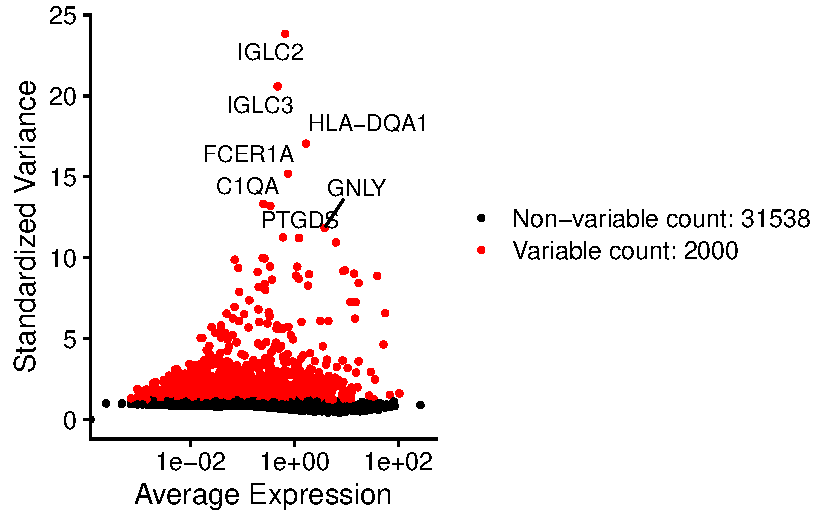
\includegraphics{citeseq_files/figure-pdf/unnamed-chunk-11-2.pdf}

}

\end{figure}

\begin{Shaded}
\begin{Highlighting}[]
\DocumentationTok{\#\# Computing nearest neighbor graph}
\NormalTok{obj }\OtherTok{\textless{}{-}} \FunctionTok{FindNeighbors}\NormalTok{(}\AttributeTok{object =}\NormalTok{ obj, }\AttributeTok{reduction =} \StringTok{"pca"}\NormalTok{, }\AttributeTok{dims =} \DecValTok{1}\SpecialCharTok{:}\DecValTok{20}\NormalTok{)}
\end{Highlighting}
\end{Shaded}

\begin{verbatim}
Computing nearest neighbor graph
\end{verbatim}

\begin{verbatim}
Computing SNN
\end{verbatim}

\begin{Shaded}
\begin{Highlighting}[]
\CommentTok{\# clustering (adjust dimensions and resolutions as desired)}
\CommentTok{\# default is Louvain clustering {-} check how it works}
\CommentTok{\# talk about resolution a bit}
\NormalTok{obj }\OtherTok{\textless{}{-}} \FunctionTok{FindClusters}\NormalTok{(}\AttributeTok{object =}\NormalTok{ obj, }\AttributeTok{resolution =} \FloatTok{0.4}\NormalTok{)}
\end{Highlighting}
\end{Shaded}

\begin{verbatim}
Modularity Optimizer version 1.3.0 by Ludo Waltman and Nees Jan van Eck

Number of nodes: 4193
Number of edges: 154360

Running Louvain algorithm...
Maximum modularity in 10 random starts: 0.9097
Number of communities: 10
Elapsed time: 0 seconds
\end{verbatim}

\begin{Shaded}
\begin{Highlighting}[]
\CommentTok{\#UMAP}
\NormalTok{obj }\OtherTok{\textless{}{-}} \FunctionTok{RunUMAP}\NormalTok{(}\AttributeTok{object =}\NormalTok{ obj, }\AttributeTok{reduction =} \StringTok{"pca"}\NormalTok{, }\AttributeTok{dims =} \DecValTok{1}\SpecialCharTok{:}\DecValTok{20}\NormalTok{)}
\end{Highlighting}
\end{Shaded}

\begin{verbatim}
Warning: The default method for RunUMAP has changed from calling Python UMAP via reticulate to the R-native UWOT using the cosine metric
To use Python UMAP via reticulate, set umap.method to 'umap-learn' and metric to 'correlation'
This message will be shown once per session
\end{verbatim}

\begin{verbatim}
14:02:33 UMAP embedding parameters a = 0.9922 b = 1.112
\end{verbatim}

\begin{verbatim}
14:02:33 Read 4193 rows and found 20 numeric columns
\end{verbatim}

\begin{verbatim}
14:02:33 Using Annoy for neighbor search, n_neighbors = 30
\end{verbatim}

\begin{verbatim}
14:02:33 Building Annoy index with metric = cosine, n_trees = 50
\end{verbatim}

\begin{verbatim}
0%   10   20   30   40   50   60   70   80   90   100%
\end{verbatim}

\begin{verbatim}
[----|----|----|----|----|----|----|----|----|----|
\end{verbatim}

\begin{verbatim}
**************************************************|
14:02:34 Writing NN index file to temp file C:\Users\ferhatay\AppData\Local\Temp\Rtmpm8JRS4\file2484f46676f
14:02:34 Searching Annoy index using 1 thread, search_k = 3000
14:02:37 Annoy recall = 100%
14:02:37 Commencing smooth kNN distance calibration using 1 thread with target n_neighbors = 30
14:02:38 Initializing from normalized Laplacian + noise (using irlba)
14:02:39 Commencing optimization for 500 epochs, with 174318 positive edges
14:02:52 Optimization finished
\end{verbatim}

\begin{Shaded}
\begin{Highlighting}[]
\CommentTok{\# you can also use the LabelClusters function to help label individual clusters}
\NormalTok{plot\_seurat\_clusters }\OtherTok{\textless{}{-}} \FunctionTok{UMAPPlot}\NormalTok{(}\AttributeTok{object =}\NormalTok{ obj, }\AttributeTok{label =} \ConstantTok{TRUE}\NormalTok{, }\AttributeTok{label.size =} \DecValTok{5}\NormalTok{) }\SpecialCharTok{+}
                          \FunctionTok{labs}\NormalTok{(}\AttributeTok{title =} \StringTok{"Initial Clusters"}\NormalTok{) }\SpecialCharTok{+}
                          \FunctionTok{theme}\NormalTok{(}\AttributeTok{plot.title =} \FunctionTok{element\_text}\NormalTok{(}\AttributeTok{hjust =} \FloatTok{0.5}\NormalTok{),}
                                \AttributeTok{axis.text =} \FunctionTok{element\_blank}\NormalTok{(),}
                                \AttributeTok{axis.ticks =} \FunctionTok{element\_blank}\NormalTok{())}
\NormalTok{plot\_seurat\_clusters}
\end{Highlighting}
\end{Shaded}

\begin{figure}[H]

{\centering 
\includegraphics{citeseq_files/figure-pdf/unnamed-chunk-15-1.pdf}

}

\end{figure}

\begin{Shaded}
\begin{Highlighting}[]
\CommentTok{\# sort by Cell\_Type and Marker if not already sorted}
\NormalTok{markers\_all }\OtherTok{\textless{}{-}} \FunctionTok{read.csv}\NormalTok{(}\AttributeTok{file =} \FunctionTok{file.path}\NormalTok{(path\_data, }\StringTok{"marker\_genes.csv"}\NormalTok{))}
\NormalTok{markers\_all }\SpecialCharTok{\%\textgreater{}\%} \FunctionTok{slice\_sample}\NormalTok{(}\AttributeTok{n =} \DecValTok{10}\NormalTok{) }\CommentTok{\# example markers}
\end{Highlighting}
\end{Shaded}

\begin{verbatim}
     Cell_Type    Marker
1            B TNFRSF13B
2            B     CXCR4
3           NK      GNLY
4          pDC      TCF4
5            B     CD79B
6            T     CAMK4
7           NK      GNLY
8            B      CD24
9     Myocytes      MYLK
10 Macrophages      CD14
\end{verbatim}

\begin{Shaded}
\begin{Highlighting}[]
\NormalTok{select\_cell\_types }\OtherTok{\textless{}{-}} \FunctionTok{c}\NormalTok{(}\StringTok{"B"}\NormalTok{, }\StringTok{"Macrophages"}\NormalTok{, }\StringTok{"mDC"}\NormalTok{, }\StringTok{"NK"}\NormalTok{, }\StringTok{"T"}\NormalTok{)}

\CommentTok{\# do features = unique(markers\_all$Marker) to use all possible features}
\NormalTok{p }\OtherTok{\textless{}{-}} \FunctionTok{DotPlot}\NormalTok{(}\AttributeTok{object =}\NormalTok{ obj,}
             \AttributeTok{features =}\NormalTok{ markers\_all }\SpecialCharTok{\%\textgreater{}\%}
\NormalTok{                          dplyr}\SpecialCharTok{::}\FunctionTok{filter}\NormalTok{(Cell\_Type }\SpecialCharTok{\%in\%}\NormalTok{ select\_cell\_types) }\SpecialCharTok{\%\textgreater{}\%}
                          \FunctionTok{distinct}\NormalTok{(Marker) }\SpecialCharTok{\%\textgreater{}\%} \FunctionTok{pull}\NormalTok{(),}
             \AttributeTok{cols =} \StringTok{"RdBu"}\NormalTok{, }\AttributeTok{col.min =} \SpecialCharTok{{-}}\DecValTok{1}\NormalTok{, }\AttributeTok{dot.scale =} \DecValTok{3}\NormalTok{, }\AttributeTok{cluster.idents =} \ConstantTok{TRUE}\NormalTok{)}

\CommentTok{\# add in the cell type information}
\CommentTok{\# if desired, you could rename the "Cell\_Type"s in the original database to be}
\CommentTok{\# more informative e.g. Natural\_Killers instead of NK}
\NormalTok{p}\SpecialCharTok{$}\NormalTok{data }\OtherTok{\textless{}{-}} \FunctionTok{left\_join}\NormalTok{(p}\SpecialCharTok{$}\NormalTok{data,}
\NormalTok{                    markers\_all }\SpecialCharTok{\%\textgreater{}\%}
\NormalTok{                      dplyr}\SpecialCharTok{::}\FunctionTok{filter}\NormalTok{(Cell\_Type }\SpecialCharTok{\%in\%}\NormalTok{ select\_cell\_types) }\SpecialCharTok{\%\textgreater{}\%}
\NormalTok{                      dplyr}\SpecialCharTok{::}\FunctionTok{rename}\NormalTok{(}\AttributeTok{features.plot =} \StringTok{"Marker"}\NormalTok{),}
                    \AttributeTok{by =} \StringTok{"features.plot"}\NormalTok{, }\AttributeTok{multiple =} \StringTok{"all"}\NormalTok{)}
\end{Highlighting}
\end{Shaded}

\begin{verbatim}
Warning in left_join(p$data, markers_all %>% dplyr::filter(Cell_Type %in% : Detected an unexpected many-to-many relationship between `x` and `y`.
i Row 24 of `x` matches multiple rows in `y`.
i Row 1 of `y` matches multiple rows in `x`.
i If a many-to-many relationship is expected, set `relationship =
  "many-to-many"` to silence this warning.
\end{verbatim}

\begin{Shaded}
\begin{Highlighting}[]
\CommentTok{\# plot}
\NormalTok{p }\SpecialCharTok{+}
  \FunctionTok{facet\_grid}\NormalTok{(}\AttributeTok{cols =} \FunctionTok{vars}\NormalTok{(Cell\_Type), }\AttributeTok{scales =} \StringTok{"free\_x"}\NormalTok{, }\AttributeTok{space =} \StringTok{"free"}\NormalTok{) }\SpecialCharTok{+}
  \FunctionTok{theme}\NormalTok{(}\AttributeTok{strip.text.x =} \FunctionTok{element\_text}\NormalTok{(}\AttributeTok{size =} \DecValTok{10}\NormalTok{)) }\SpecialCharTok{+} \FunctionTok{RotatedAxis}\NormalTok{()}
\end{Highlighting}
\end{Shaded}

\begin{figure}[H]

{\centering 
\includegraphics{citeseq_files/figure-pdf/unnamed-chunk-17-1.pdf}

}

\end{figure}

\begin{Shaded}
\begin{Highlighting}[]
\CommentTok{\# you have to change the default assay for the dot plot}
\FunctionTok{DefaultAssay}\NormalTok{(}\AttributeTok{object =}\NormalTok{ obj) }\OtherTok{\textless{}{-}} \StringTok{"ADT"}

\FunctionTok{DotPlot}\NormalTok{(}\AttributeTok{object =}\NormalTok{ obj,}
        \AttributeTok{features =} \FunctionTok{rownames}\NormalTok{(}\FunctionTok{GetAssayData}\NormalTok{(}\AttributeTok{object =}\NormalTok{ obj, }\AttributeTok{assay =} \StringTok{"ADT"}\NormalTok{,}
                                         \AttributeTok{slot =} \StringTok{"counts"}\NormalTok{)),}
        \AttributeTok{cols =} \StringTok{"RdBu"}\NormalTok{, }\AttributeTok{col.min =} \SpecialCharTok{{-}}\DecValTok{1}\NormalTok{, }\AttributeTok{dot.scale =} \DecValTok{3}\NormalTok{, }\AttributeTok{cluster.idents =} \ConstantTok{TRUE}\NormalTok{) }\SpecialCharTok{+}
  \FunctionTok{RotatedAxis}\NormalTok{()}
\end{Highlighting}
\end{Shaded}

\begin{figure}[H]

{\centering 
\includegraphics{citeseq_files/figure-pdf/unnamed-chunk-18-1.pdf}

}

\end{figure}

\begin{Shaded}
\begin{Highlighting}[]
\CommentTok{\# reset the default}
\FunctionTok{DefaultAssay}\NormalTok{(}\AttributeTok{object =}\NormalTok{ obj) }\OtherTok{\textless{}{-}} \StringTok{"RNA"}
\end{Highlighting}
\end{Shaded}

\begin{Shaded}
\begin{Highlighting}[]
\FunctionTok{FeaturePlot}\NormalTok{(}\AttributeTok{object =}\NormalTok{ obj,}
            \AttributeTok{features =} \FunctionTok{c}\NormalTok{(}\StringTok{"MS4A1"}\NormalTok{, }\StringTok{"CD14"}\NormalTok{, }\CommentTok{\# MS4A1 is another name for CD20}
                         \StringTok{"NKG7"}\NormalTok{, }\StringTok{"IL3RA"}\NormalTok{, }\StringTok{"CD3D"}\NormalTok{, }\StringTok{"IL7R"}\NormalTok{), }
            \AttributeTok{min.cutoff =} \DecValTok{0}\NormalTok{, }\AttributeTok{label =} \ConstantTok{TRUE}\NormalTok{, }\AttributeTok{label.size =} \DecValTok{3}\NormalTok{,}
            \AttributeTok{ncol =} \DecValTok{3}\NormalTok{, }\AttributeTok{raster =} \ConstantTok{FALSE}\NormalTok{)}
\end{Highlighting}
\end{Shaded}

\begin{figure}[H]

{\centering 
\includegraphics{citeseq_files/figure-pdf/unnamed-chunk-20-1.pdf}

}

\end{figure}

\begin{Shaded}
\begin{Highlighting}[]
\FunctionTok{VlnPlot}\NormalTok{(}\AttributeTok{object =}\NormalTok{ obj,}
        \AttributeTok{features =} \FunctionTok{c}\NormalTok{(}\StringTok{"CD3{-}TotalSeqB"}\NormalTok{, }\StringTok{"CD14{-}TotalSeqB"}\NormalTok{, }\StringTok{"CD20{-}TotalSeqB"}\NormalTok{,}
                     \StringTok{"CD335{-}TotalSeqB"}\NormalTok{),}
        \AttributeTok{pt.size =} \DecValTok{0}\NormalTok{, }\AttributeTok{assay =} \StringTok{"ADT"}\NormalTok{, }\AttributeTok{ncol =} \DecValTok{2}\NormalTok{) }\SpecialCharTok{\&}
  \FunctionTok{theme}\NormalTok{(}\AttributeTok{plot.title =} \FunctionTok{element\_text}\NormalTok{(}\AttributeTok{size =} \DecValTok{10}\NormalTok{),}
        \AttributeTok{axis.text.x =} \FunctionTok{element\_text}\NormalTok{(}\AttributeTok{angle =} \DecValTok{0}\NormalTok{, }\AttributeTok{hjust =} \FloatTok{0.5}\NormalTok{),}
        \AttributeTok{axis.title.x =} \FunctionTok{element\_blank}\NormalTok{())}
\end{Highlighting}
\end{Shaded}

\begin{figure}[H]

{\centering 
\includegraphics{citeseq_files/figure-pdf/unnamed-chunk-21-1.pdf}

}

\end{figure}

\begin{Shaded}
\begin{Highlighting}[]
\CommentTok{\# mDC = myeloid dendritic cells}
\CommentTok{\# pDC = plasmacytoid dendritic cells}
\NormalTok{obj\_annotations }\OtherTok{\textless{}{-}} \FunctionTok{rbind}\NormalTok{(}\FunctionTok{c}\NormalTok{(}\StringTok{"0"}\NormalTok{, }\StringTok{"Macrophages/mDCs"}\NormalTok{), }\CommentTok{\# difficult to separate}
                         \FunctionTok{c}\NormalTok{(}\StringTok{"1"}\NormalTok{, }\StringTok{"T Cells"}\NormalTok{),}
                         \FunctionTok{c}\NormalTok{(}\StringTok{"2"}\NormalTok{, }\StringTok{"T Cells"}\NormalTok{),}
                         \FunctionTok{c}\NormalTok{(}\StringTok{"3"}\NormalTok{, }\StringTok{"T Cells"}\NormalTok{),}
                         \FunctionTok{c}\NormalTok{(}\StringTok{"4"}\NormalTok{, }\StringTok{"Natural Killers"}\NormalTok{),}
                         \FunctionTok{c}\NormalTok{(}\StringTok{"5"}\NormalTok{, }\StringTok{"B Cells"}\NormalTok{),}
                         \FunctionTok{c}\NormalTok{(}\StringTok{"6"}\NormalTok{, }\StringTok{"Macrophages/mDCs"}\NormalTok{), }\CommentTok{\# difficult to separate}
                         \FunctionTok{c}\NormalTok{(}\StringTok{"7"}\NormalTok{, }\StringTok{"Macrophages/mDCs"}\NormalTok{), }\CommentTok{\# difficult to separate}
                         \FunctionTok{c}\NormalTok{(}\StringTok{"8"}\NormalTok{, }\StringTok{"T Cells"}\NormalTok{), }\CommentTok{\# faint signal}
                         \FunctionTok{c}\NormalTok{(}\StringTok{"9"}\NormalTok{, }\StringTok{"pDCs"}\NormalTok{))}
\FunctionTok{colnames}\NormalTok{(obj\_annotations) }\OtherTok{\textless{}{-}} \FunctionTok{c}\NormalTok{(}\StringTok{"Cluster"}\NormalTok{, }\StringTok{"CellType"}\NormalTok{)}
\NormalTok{obj\_annotations }\OtherTok{\textless{}{-}} \FunctionTok{data.frame}\NormalTok{(obj\_annotations)}
\NormalTok{obj\_annotations}
\end{Highlighting}
\end{Shaded}

\begin{verbatim}
   Cluster         CellType
1        0 Macrophages/mDCs
2        1          T Cells
3        2          T Cells
4        3          T Cells
5        4  Natural Killers
6        5          B Cells
7        6 Macrophages/mDCs
8        7 Macrophages/mDCs
9        8          T Cells
10       9             pDCs
\end{verbatim}

\begin{Shaded}
\begin{Highlighting}[]
\CommentTok{\# save the annotations as a csv if you\textquotesingle{}d like}
\CommentTok{\# write.csv(obj\_annotations, file = file.path(path\_data, "obj\_annotations.csv"))}

\CommentTok{\# prepare the annotation information}
\NormalTok{annotations }\OtherTok{\textless{}{-}} \FunctionTok{setNames}\NormalTok{(obj\_annotations}\SpecialCharTok{$}\NormalTok{CellType, obj\_annotations}\SpecialCharTok{$}\NormalTok{Cluster)}
\NormalTok{annotations}
\end{Highlighting}
\end{Shaded}

\begin{verbatim}
                 0                  1                  2                  3 
"Macrophages/mDCs"          "T Cells"          "T Cells"          "T Cells" 
                 4                  5                  6                  7 
 "Natural Killers"          "B Cells" "Macrophages/mDCs" "Macrophages/mDCs" 
                 8                  9 
         "T Cells"             "pDCs" 
\end{verbatim}

\begin{Shaded}
\begin{Highlighting}[]
\CommentTok{\# relabel the Seurat clusters}
\CommentTok{\# Idents(obj) \textless{}{-} "seurat\_clusters"}
\NormalTok{obj }\OtherTok{\textless{}{-}} \FunctionTok{RenameIdents}\NormalTok{(}\AttributeTok{object =}\NormalTok{ obj, annotations)}

\CommentTok{\# alphabetize the cell types}
\FunctionTok{Idents}\NormalTok{(obj) }\OtherTok{\textless{}{-}} \FunctionTok{factor}\NormalTok{(}\FunctionTok{Idents}\NormalTok{(}\AttributeTok{object =}\NormalTok{ obj), }\AttributeTok{levels =} \FunctionTok{sort}\NormalTok{(}\FunctionTok{levels}\NormalTok{(obj)))}

\CommentTok{\# useful metadata (e.g. if you want to have multiple annotation sets)}
\NormalTok{obj[[}\StringTok{"annotated\_clusters"}\NormalTok{]] }\OtherTok{\textless{}{-}} \FunctionTok{Idents}\NormalTok{(}\AttributeTok{object =}\NormalTok{ obj)}

\CommentTok{\# save the processed and annotated Seurat object}
\CommentTok{\# saveRDS(obj, file = file.path(path\_data, "tenx\_pbmc5k\_CITEseq\_annotated.rds"))}

\CommentTok{\# info about the clusters}
\NormalTok{obj\_annotations }\SpecialCharTok{\%\textgreater{}\%}
  \FunctionTok{group\_by}\NormalTok{(CellType) }\SpecialCharTok{\%\textgreater{}\%}
  \FunctionTok{transmute}\NormalTok{(}\AttributeTok{Clusters =} \FunctionTok{paste0}\NormalTok{(Cluster, }\AttributeTok{collapse =} \StringTok{", "}\NormalTok{)) }\SpecialCharTok{\%\textgreater{}\%}
  \FunctionTok{distinct}\NormalTok{() }\SpecialCharTok{\%\textgreater{}\%}
  \FunctionTok{arrange}\NormalTok{(CellType)}
\end{Highlighting}
\end{Shaded}

\begin{verbatim}
# A tibble: 5 x 2
# Groups:   CellType [5]
  CellType         Clusters  
  <chr>            <chr>     
1 B Cells          5         
2 Macrophages/mDCs 0, 6, 7   
3 Natural Killers  4         
4 T Cells          1, 2, 3, 8
5 pDCs             9         
\end{verbatim}

\begin{Shaded}
\begin{Highlighting}[]
\CommentTok{\# plot ADT information on top as an example}

\FunctionTok{FeaturePlot}\NormalTok{(}\AttributeTok{object =}\NormalTok{ obj, }\AttributeTok{features =} \StringTok{"adt\_CD19{-}TotalSeqB"}\NormalTok{,}
            \AttributeTok{label =} \ConstantTok{TRUE}\NormalTok{, }\AttributeTok{label.size =} \DecValTok{3}\NormalTok{, }\AttributeTok{ncol =} \DecValTok{1}\NormalTok{, }\AttributeTok{raster =} \ConstantTok{FALSE}\NormalTok{)}
\end{Highlighting}
\end{Shaded}

\begin{figure}[H]

{\centering 
\includegraphics{citeseq_files/figure-pdf/unnamed-chunk-23-1.pdf}

}

\end{figure}

The \texttt{echo:\ false} option disables the printing of code (only
output is displayed).



\end{document}
